\chapter{Introduction}
\label{chap:introduction}
This is a citation: \cite{patchCore2022}


This is a figure: 

\begin{figure}[ht]
    \centering
    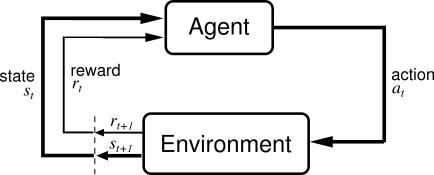
\includegraphics[width=.5\textwidth]{figures/AgentEnviornment.png}
    \caption{I am a caption}
    \label{fig:my_label}
\end{figure}



- It is important to note somewhere in the paper that we are dealing with very high variance in our ensemble since we only have 5 models ish


\section{Begin Intro}
In recent years, image anomaly detection has become significantly more important among many scientific communities, especially in industrial applications. This is no surprise, considering the
amount of mechanically manufactured parts in factories all over the world. Since in most parts of the world, manufactured items undergo rather strict regulations and are expected to work
in real case scenarios, there is a need for sufficient quality control, that is rising with the amount of produced components. A long time ago, it has come to a point where human based quality 
checks are not adequate anymore for the production volume, which has led to computer solutions for the problem. Generally speaking, anomaly detection has first been proposed in 1986 for 
intrusion detection systems(referenz). While the methods and modalities may change, the high level idea stays the same: Detecting data that deviates from a set standard to a degree that is becoming
problematatic regarding the own requirements(letzer part maybe neu formulieren). Besides many approaches that were used over the years, deep learning approaches for image anomaly detection have
become very popular lately. A likely reason for this are impressively high performance scores with state of the art models achieving an area under the receiver operateor curve of around 0.96 and 
sometimes even more.
It is difficult to say what the first deep learning approaches to this topic were(fact checking), but a notable milestone is definetly Bergmann 2021(Referenz). Among blabla, they introduced
the MVTecAD dataset which is used widely and serves as a dataset to benchmark on for nearly every IAD paper released afterwards. - Übergang benötigt

\section{Table Test Viz}

This is a table:
\begin{table}[htbp]
    \tiny
    \centering
    \begin{tabularx}{\textwidth}{|X|X|X|}%{|c|p{5cm}|p{5cm}|p{5cm}|}
        \hline
        \textbf{Metric/Level} & \textbf{Formula} & \textbf{Remarks/Usage} \\
        \hline
        Precision (P) $\uparrow$ & $P = TP/(TP + FP)$ & True Positive (TP), False Positive (FP) \\
        \hline
        Recall (R) $\uparrow$ & $R = TP/(TP + FN)$ & False Negative (FN), True Positive Rate (TPR) \\
        \hline
        True Positive Rate (TPR) $\uparrow$ & $TPR = TP/(TP + TN)$ & True Negative (TN) \\
        \hline
        False Positive Rate (FPR) $\downarrow$ & $FPR = FP/(FP + TN)$ & True Negative (TN) \\
        \hline
        Area Under the Receiver Operating Characteristic curve (AU-ROC) $\uparrow$ & $ \int_{0}^{1} (TPR) \: d(FPR)$ & Classification \\
        \hline
        Area Under Precision-Recall (AU-PR) $\uparrow$ & $\int_{0}^{1} P \: d(R)$ & Localization, Segmentation \\
        \hline
        Per-Region Overlap (PRO) $\uparrow$ & $PRO = \frac{1}{N} \sum_{i} \sum_{k} \frac{P_i \cap C_{i,k}}{C_{i,k}}$ & Total ground-truth number (\(N\)), Predicted abnormal pixels (\(P\)), Defect ground-truth regions (\(C\)) \\
        \hline
        Saturated Per-Region Overlap (sPRO) $\uparrow$ & $sPRO(P) = \frac{1}{m} \sum_{i=1}^{m} \min(\frac{A_i \cap P}{s_i}, 1)$ & Total ground-truth number (\(m\)), Predicted abnormal pixels (\(P\)), Defect ground-truth regions (\(A\)), Corresponding saturation thresholds (\(s\)) \\
        \hline
        F1 Score $\uparrow$ & $F1 = 2(P \cdot R)/(P + R)$ & Classification \\
        \hline
        Intersection over Union (IoU) $\uparrow$ & $IoU = (H \cap G)/(H \cup G)$ & Prediction (H), Ground truth (G)/ Localization, Segmentation \\
        \hline
    \end{tabularx}
    \caption{Description of metrics}
    \label{tab:metrics}
\end{table}






\section{Contributions}
This work builds upon the researched anomaly detection methods that were established as state of the art over the last years. Papers like survey1 and survey2 provide extensive overviews of all SOTA methods,
including the ones mentioned in this thesis. The main contributions thus are:
1. Creating a pipeline for anomaly detection experiments and inference, utilizing existing IAD approaches. 
2. Introducing three??? new categories for the mvtec(LOCO) dataset for anomaly detection experiments.
3. Researching anomaly detection performance on multi perspective datasets. ???
4. Research on incresed robustness in anomaly detection using feature map level ensembles.

The contributions mentioned firstly benefit faster research with a streamlined(synonym) experiment setup. Furthermore they give more insight into the capabilities of existing methods in a 
industrial setting and thus also provide a more various and practical setting than the prior categories in the mvtec(zitat) dataset. The same methods are also testet on their limitations 
regarding logical anomalies which is(synonym) a relevant aspect of anomaly detection in current manufacturing quality control. Lastly through the use of a robust ensemble approach for heterogeneous 
classifers, this opens up possibilities for expanding the field of application of SOTA IAD methods to other domains with robust performance and may also produce more usable results in real world 
IAD settings.

%Experiment on the performance of different ensemble methods for IAD, including utilizing majority voting, stacking, CAWPE and (die anderen ensemble paper von discord zitieren).

The above contributions can be used as basis for industrial usage, aswell as a basis for future contributions on ensemble methods in the IAD space. Moreover it gives further insight on the
efficiency of SOTA IAD methods on different kinds of data than the previous synthetic settings.



-- in my work i contribute the following things:
- pipeline to infer new images on different algorithms and compare them
-> pipeline is industry focussed for benefits of the guys where i write my thesis

- research on multi perspective detection

- research of ensemble output learning to enhance individual network performance
-> simple network over 5-6 outputs

- introduction of very new dataset categories in style of mvtec LOCO dataset

